% Meta: ~800 palabras
\section{Resultados y discusión}

\subsection{Desempeño de la mezcla}

La tabla~\ref{tab:candidatos} resume la comparación anidada. Donde se califica, el ensamble y la mezcla empatan en RMSE (0.508 t/ha) y en $R^{2}$ (0.64). La mezcla tiene mejor MAE (0.354 frente a 0.362) y un sesgo de +0.005 t/ha. Predecir el promedio de las parcelas de entrenamiento da un RMSE de 0.846: la mezcla recorta ese error en cerca de un 40\,\%. El modelo de solo longitud queda cerca en la estratificada (0.525) y es el mejor en LOMO (0.539), lo que confirma que la geografía carga mucha señal. El ensamble, en cambio, se degrada al sacar un municipio (RMSE 0.722, sesgo $-0.102$). La mezcla queda en medio (0.595, sesgo $-0.013$): no pierde donde se califica y recorta casi la mitad de la caída del ensamble en zona nueva. Por ese equilibrio se firmó como entrega. La figura~\ref{fig:dispersion} muestra las 138 predicciones fuera de muestra frente al valor observado; la figura~\ref{fig:residuales}, los residuales.

\begin{table}[ht]
\centering
\caption{Tres candidatos, mismas 138 parcelas. RMSE, MAE y sesgo en t/ha.}
\label{tab:candidatos}
\small
\begin{tabular}{lrrrrrr}
\toprule
 & \multicolumn{3}{c}{Estratificada} & \multicolumn{2}{c}{LOMO} \\
\cmidrule(lr){2-4}\cmidrule(lr){5-6}
Candidato & RMSE & MAE & $R^{2}$ & RMSE & Sesgo \\
\midrule
Ensamble (121 var.) & 0.508 & 0.362 & 0.64 & 0.722 & $-0.102$ \\
Solo longitud & 0.525 & 0.364 & 0.62 & 0.539 & +0.077 \\
Mezcla (entrega) & 0.508 & 0.354 & 0.64 & 0.595 & $-0.013$ \\
\bottomrule
\end{tabular}
\end{table}

\begin{figure}[ht]
\centering
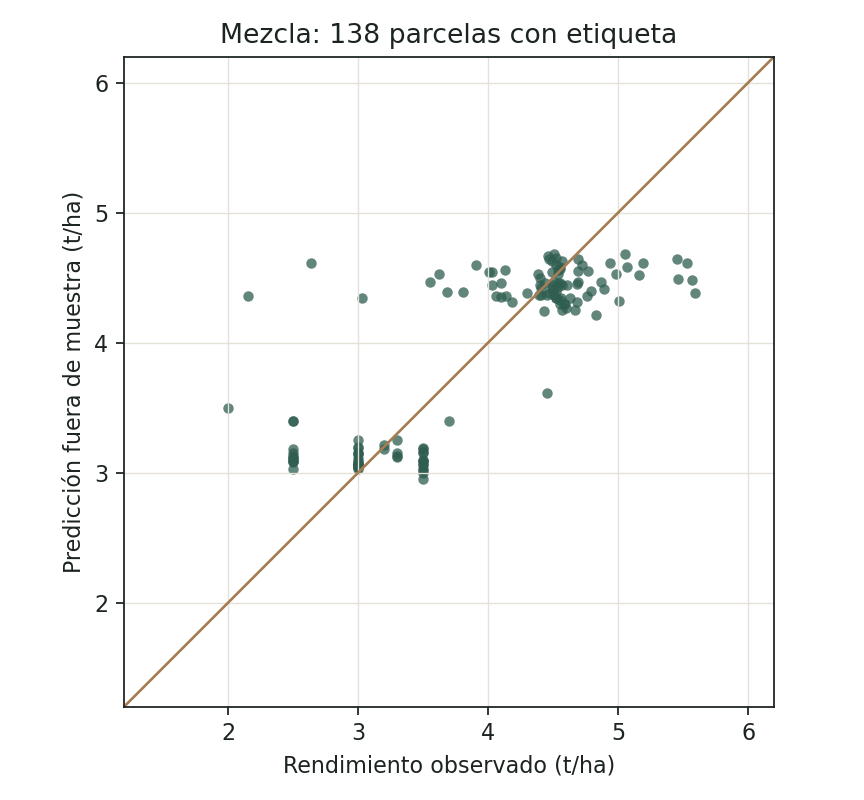
\includegraphics[width=0.72\textwidth]{figuras/dispersion.png}
\caption{Observado contra predicción fuera de muestra de la mezcla.}
\label{fig:dispersion}
\end{figure}

\begin{figure}[ht]
\centering
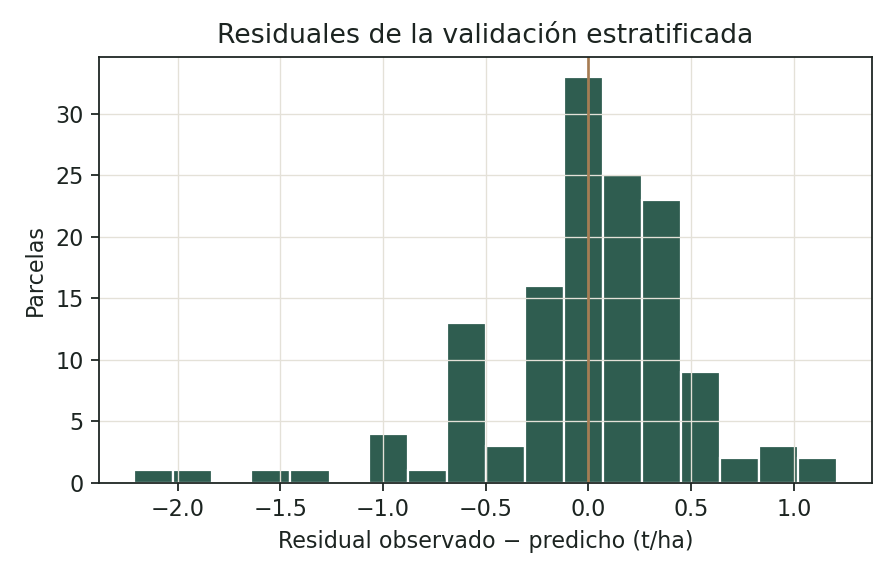
\includegraphics[width=0.78\textwidth]{figuras/residuales.png}
\caption{Distribución de residuales de la validación estratificada.}
\label{fig:residuales}
\end{figure}

La prueba del ganador del superciclo, hecha con los mismos pliegues, no cambió la firma. Ese LightGBM, de 13 variables y con nitrógeno de SoilGrids más edafología, obtuvo un RMSE estratificado de 0.582 t/ha, peor que la mezcla. Con Optuna anidado bajó a 0.547 y, mezclado con el ensamble, a 0.520. En ningún caso se cumplieron a la vez la mejora de 0.010 t/ha, un LOMO no peor y un intervalo bootstrap por debajo de cero. Los datos externos no compraron precisión en el conjunto que se califica.

Al dejar un municipio fuera, el error de la mezcla no es uniforme (figura~\ref{fig:lomo}). Con al menos cinco parcelas, Almoloya queda en 0.28 t/ha ($n=10$), Cuautepec de Hinojosa en 0.32 ($n=5$), Calpulalpan en 0.44 ($n=30$), Chignahuapan en 0.61 ($n=71$) y Singuilucan en 0.90 ($n=16$). Chignahuapan concentra la mitad de la muestra; Singuilucan es el punto débil. El agregado LOMO de 0.595 es un promedio exigente, no un error típico de cada municipio. La figura omite municipios de menos de cinco parcelas.

\begin{figure}[ht]
\centering
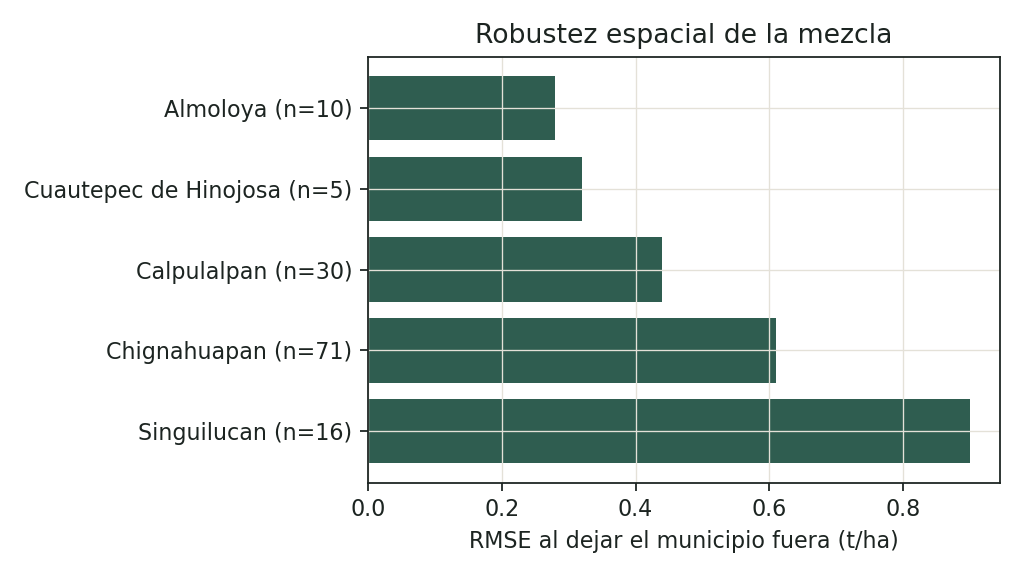
\includegraphics[width=0.82\textwidth]{figuras/lomo_municipio.png}
\caption{RMSE de la mezcla al excluir cada municipio con al menos cinco parcelas.}
\label{fig:lomo}
\end{figure}

\subsection{Preguntas guía}

Las respuestas usan el valor absoluto medio de SHAP del LightGBM del ensamble. No describen la mezcla completa.

\textit{¿Qué índice pesa más?} Al sumar las contribuciones de las variables derivadas de cada índice, el mayor es el NDVI (0.081 t/ha), seguido del NDDI (0.072) y del LAI (0.050). Dentro del NDVI, la velocidad de senescencia (0.049) supera al valor máximo (0.002). El pico de verdor casi no discrimina; la dinámica del ciclo sí. La figura~\ref{fig:shap} agrupa esas familias.

\textit{¿Qué variable climática pesa más?} La lluvia de mayo (\texttt{prec\_mm\_m05}) concentra 0.268 t/ha de $|$SHAP$|$, muy por encima de la lluvia de abril (0.047), la temperatura máxima de abril (0.026) y la mínima de abril (0.021). La familia climática suma 0.381, la mayor de todas. Ese peso no demuestra que la lluvia de mayo cause el rendimiento: el píxel climático mide unos 5 km y puede estar actuando como indicador de zona, del mismo modo que la longitud.

\textit{¿Qué combinación funciona mejor?} La ablación, con el mismo esquema estratificado, ordena los bloques así: solo clima, 0.507 t/ha (16 variables); todas las variables, 0.508 (121); clima más satélite, 0.512 (99); topografía y ubicación, 0.514 (16); clima y ubicación, 0.523 (32); solo satélite, 0.613 (83). El mejor bloque puntual es el clima. La diferencia con el modelo completo es de 0.001 t/ha, dentro del ruido de 0.010. El satélite solo, sin clima, es claramente peor. La mezcla se quedó con las 121 variables porque el empate no justifica tirar el satélite, que sí aporta en la ficha y en la lectura agronómica, y porque el criterio de entrega miraba también el LOMO, no solo esta ablación. La figura~\ref{fig:ablacion} muestra la comparación.

\begin{figure}[ht]
\centering
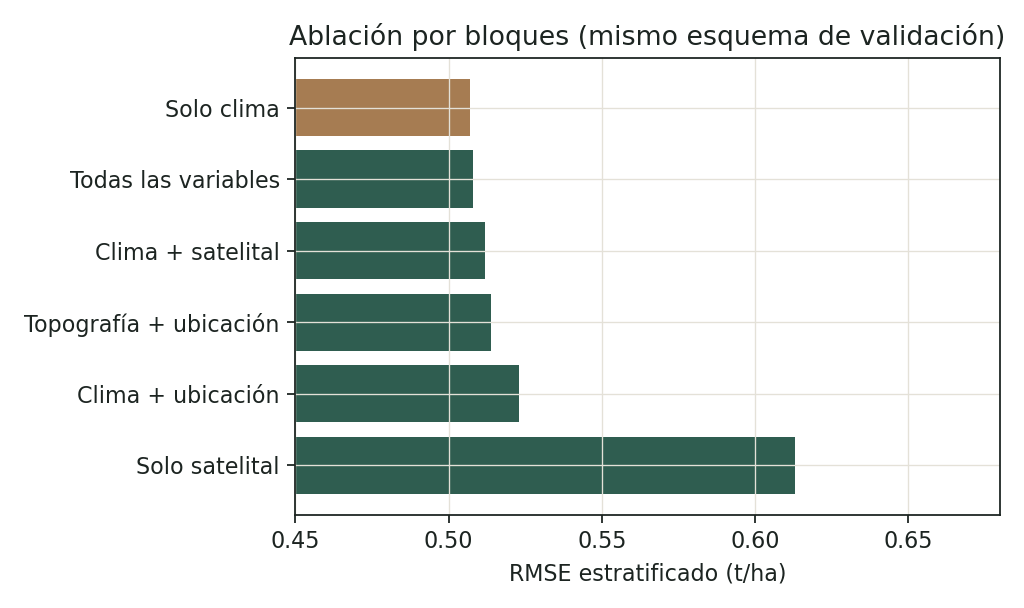
\includegraphics[width=0.86\textwidth]{figuras/ablacion.png}
\caption{RMSE estratificado por bloque de variables.}
\label{fig:ablacion}
\end{figure}

\begin{figure}[ht]
\centering
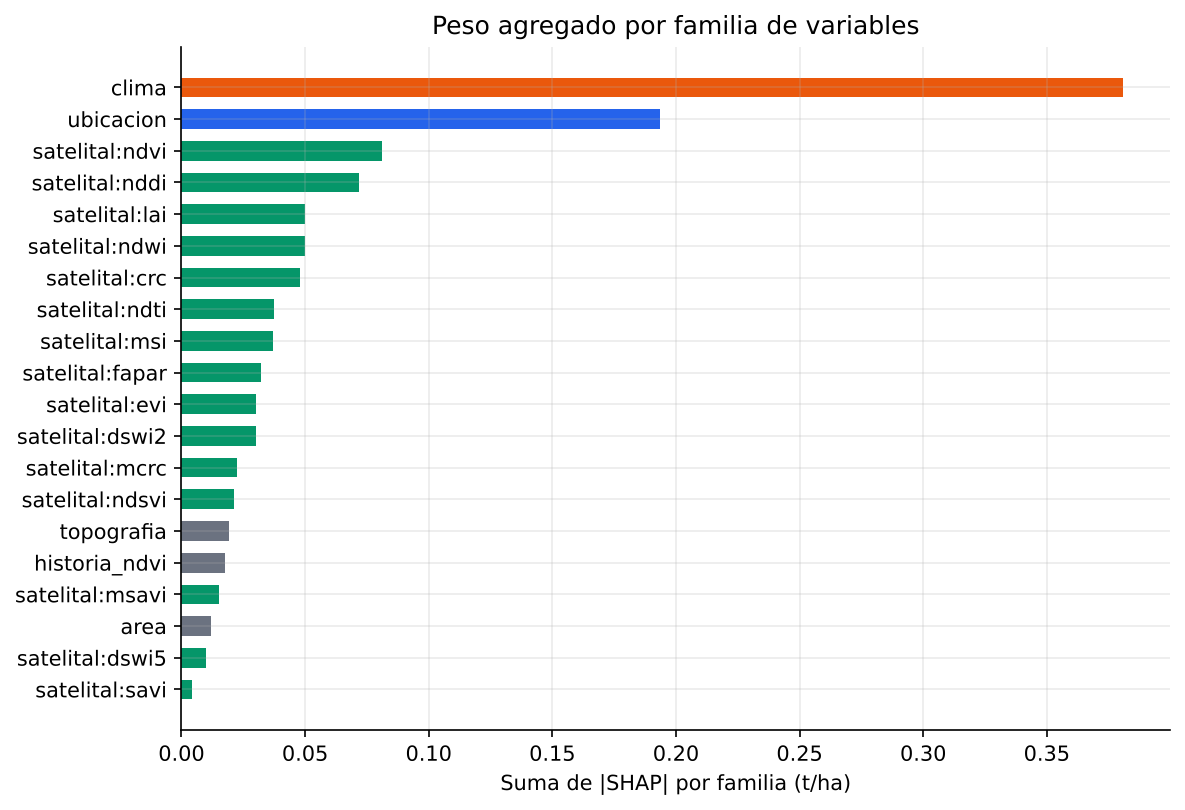
\includegraphics[width=0.92\textwidth]{figuras/fig_shap_familias.png}
\caption{Contribución $|$SHAP$|$ por familia en el LightGBM del ensamble (peso 1/6 de la mezcla).}
\label{fig:shap}
\end{figure}

\subsection{Límites}

Las 59 predicciones de entrega están calculadas y se consultan en el dashboard, pero este reporte no les asigna un error: la etiqueta la resguarda el comité. Publicar un RMSE sobre ellas sería inventar la calificación.

El modelo vio una sola temporada. Fuera de esta región la longitud no es transferible: habría que reentrenar con rendimientos locales. En el simulador, el efecto climático aparece atenuado a la mitad porque la longitud no se mueve. En Tlaxcala el rendimiento observado toma pocos valores, lo que parece una estimación por zona más que una medición parcela a parcela. La herramienta apoya la consulta; no sustituye la evaluación crediticia ni una visita de campo.
